\section*{Đề kiểm tra Chương 8}
\subsection*{Đề số 2}
\setcounter{ex}{0}\setcounter{bt}{0}
\Opensolutionfile{ans}[ans/ans-KT-802]
\noindent\textbf{I. PHẦN TRẮC NGHIỆM}
\begin{ex}%[Hữu Bình - BG Toán 10]%[1D2Y1-1]
	Trên giá sách có $ 8 $ quyển sách Văn và $ 10 $ quyển sách Toán, các quyển này đôi một phân
	biệt. Hỏi có bao nhiêu cách chọn ra $ 1 $ quyển sách trên giá?
	\choice
	{$ 80 $}
	{$ 10 $}
	{$ 8 $}
	{\True $ 18 $}
	\loigiai{
		\begin{itemize}
			\item Số cách chọn 1 quyển sách Văn là $ 8 $.
			\item  Số cách chọn $ 1 $ quyển sách Toán là $ 10 $.
		\end{itemize}	
		Số cách chọn 1 quyển sách là $ 8+10=18 $ cách.
	}
\end{ex}

\begin{ex}%[Hữu Bình - BG Toán 10]%[1D2Y1-1]
	Một bình đựng $4$ viên bi đỏ khác nhau và $3$ viên bi xanh khác nhau. Hỏi có tất cả bao nhiêu cách lấy ra $2$ viên bi từ bình đó?
	\choice
	{$18$}
	{\True $21$}
	{$42$}
	{$10$}
	\loigiai{Số cách lấy bi là $\mathrm{C}^2_{3+4}=21.$}
\end{ex}
\begin{ex}%[Hữu Bình - BG Toán 10]%[1D2Y1-1]
	Trong $1$ lớp có $15$ bạn nam và $17$ bạn nữ. Có bao nhiêu cách chọn 1 bạn làm lớp trưởng?	
	\choice
	{$30$}
	{\True $32$}
	{$17$}
	{$15$}
	\loigiai
	{
		Số cách chọn 1 bạn làm lớp trưởng là $\mathrm{C}_{32}^1=32$.
	}
\end{ex}

\begin{ex}%[Hữu Bình - BG Toán 10]%[1D2Y1-1]
	Có $8$ quyển sách khác nhau và $6$ quyển vở khác nhau. Số cách chọn một trong các quyển đó là
	\choice
	{$6$}
	{$8$}
	{\True $14$}
	{$48$}
	\loigiai{
		Ta có $8$ cách chọn lấy $1$ quyển sách, có $6$ cách chọn lấy một quyển vở. \\
		Số cách chọn một trong các quyển đó là $14$ cách.
	}
\end{ex}
\begin{ex}%[Hữu Bình - BG Toán 10]%[1D2B1-2]
	Có $3$ kiểu mặt đồng hồ đeo tay (vuông, tròn, elip) và $4$ kiểu dây (kim loại, da, vải và nhựa). Hỏi có bao nhiêu cách chọn một chiếc đồng hồ gồm một mặt và một dây?
	\choice
	{$16$}
	{$4$}
	{$7$}
	{\True $12$}
	\loigiai{
		Chọn $1$ kiểu mặt từ $3$ kiểu mặt có $3$ cách.\\
		Chọn $1$ kiểu dây từ $4$ kiểu dây có $4$ cách.\\
		Vậy theo quy tắc nhân có $12$ cách chọn $1$ chiếc đồng hồ gồm một mặt và một dây.}
\end{ex}




\begin{ex}%[Hữu Bình - BG Toán 10]%[1D2B1-2]
	Trong mặt phẳng, cho một đa giác lồi có 20 cạnh. Số đường chéo của đa giác là
	\choice
	{360}
	{380}
	{190}
	{\True 170}
	\loigiai{
		Từ mỗi đỉnh của đa giác ta kẻ được $17$ đường chéo.\\
		Từ $20$ đỉnh kẻ được $17\cdot20=340$ đường chéo.\\
		Tuy nhiên, theo cách vẽ ở trên thì mỗi đường chéo của đa giác được kẻ 2 lần.\\
		Vậy số đường chéo của đa giác là $\dfrac{340}{2}=170$.
	}
\end{ex}

\begin{ex}%[Hữu Bình - BG Toán 10]%[1D2B1-2]
	Từ các chữ số $0$, $1$, $2$, $3$, $4$, $5$, $6$ lập được bao nhiêu số tự nhiên có $4$ chữ số?
	\choice
	{\True $2058$}
	{$2401$}
	{$720$}
	{$840$}
	\loigiai{
		Gọi số có $4$ chữ số cần lập là $\overline{abcd}$.
		\begin{itemize}
			\item $a\neq 0\Rightarrow$ có $6$ cách chọn $a$.
			\item mỗi chữ số $b$, $c$, $d$ có $7$ cách chọn.
		\end{itemize}
		Vậy có $6\cdot 7^3=2058$ cách.	
	}
\end{ex}

\begin{ex}%[Hữu Bình - BG Toán 10]%[1D2B1-2]
	Trong một lớp có $18$ bạn nam, $12$ bạn nữ. Hỏi có bao nhiêu cách chọn hại bạn trong đó có một nam và một nữ đi dự Đại hội?
	\choice
	{$18$}
	{\True $216$}
	{$12$}
	{$30$}
	\loigiai{
		Chọn một bạn nam trong $18$ bạn  nam suy ra có $18$ cách.\\
		Chọn một bạn nữ trong $12$ bạn nữ suy ra có $12$ cách.\\
		Theo quy tắc nhân ta có số cách chọn thỏa mãn yêu cầu bài toán là $18\cdot12=216$ cách.
	}
\end{ex}

\begin{ex}%[Hữu Bình - BG Toán 10]%%[1D2B1-2]
	Cho $A=\{1;2;3;4;5\}$. Từ $A$ có thể lập được bao nhiêu số tự nhiên có $2$ chữ số khác nhau ?
	\choice
	{$5^2$}
	{\True $20$}
	{$25$}
	{$2^5$}
	\loigiai{
		+ Chọn $2$ chữ số khác nhau trong $5$ chữ số và có phân biệt thứ tự giữa chúng, ta được $\mathrm{A}_5^2=20$ số.}
\end{ex}


\begin{ex}%[Hữu Bình - BG Toán 10]%[1D2Y1-3]
	Có bao nhiêu hình vuông trong hình dưới đây?
	\begin{center}
		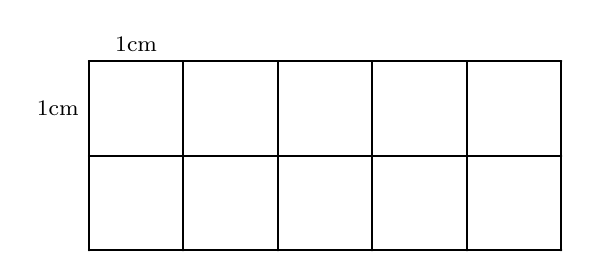
\begin{tikzpicture}[>=stealth,line join=round,line cap=round,font=\footnotesize,scale=0.6]
			\coordinate (A) at (0,0);
			\coordinate (B) at (2,0);
			\coordinate (C) at (4,0);
			\coordinate (D) at (6,0);
			\coordinate (E) at (8,0);
			\coordinate (F) at (10,0);
			\coordinate (A-1) at (0,-2);
			\coordinate (F-1) at (10,-2);
			\coordinate (A-2) at (0,-4);
			\coordinate (B-2) at (2,-4);
			\coordinate (C-2) at (4,-4);
			\coordinate (D-2) at (6,-4);
			\coordinate (E-2) at (8,-4);
			\coordinate (F-2) at (10,-4);
			\draw[line width=0.7pt,black] (A)--(F);
			\draw[line width=0.7pt,black] (A-1)--(F-1);
			\draw[line width=0.7pt,black] (A-2)--(F-2);
			\draw[line width=0.7pt,black] (A)--(A-2);
			\draw[line width=0.7pt,black] (B)--(B-2);
			\draw[line width=0.7pt,black] (C)--(C-2);
			\draw[line width=0.7pt,black] (D)--(D-2);
			\draw[line width=0.7pt,black] (E)--(E-2);
			\draw[line width=0.7pt,black] (F)--(F-2);
			\draw[line width=0.7pt,black] (A)--(B)node[above,pos=0.5]{1cm};
			\draw[line width=0.7pt,black] (A)--(A-1)node[left,pos=0.5]{1cm};
		\end{tikzpicture}
	\end{center}
	\choice
	{\True $14$}
	{$12$}
	{$10$}
	{$5$}
	\loigiai{
		Gọi $A$ là tập hợp hình vuông có cạnh $1$ cm.\\
		$B$ là tập hợp hình vuông có cạnh $2$ cm.\\
		$A$ và $B$ là hai tập hợp rời nhau.\\
		Số hình vuông trong hình là $n(A\cup B)=n(A)+n(B)=10+4=14$.}
\end{ex}

\begin{ex}%[Hữu Bình - BG Toán 10]%[1D2B1-3]
	Bình $A$ chứa $3$ quả cầu xanh, $4$ quả cầu đỏ và $5$ quả cầu trắng. Bình $B$ chứa $4$ quả cầu xanh, $3$ quả cầu đỏ và $6$ quả cầu trắng. Bình $C$ chứa $5$ quả cầu xanh, $5$ quả cầu đỏ và $2$ quả cầu trắng. Từ mỗi bình lấy ra một quả cầu. Có bao nhiêu cách lấy để cuối cùng được $3$ quả có màu giống nhau?
	\choice
	{$150$}
	{\True $180$}
	{$60$}
	{$120$}
	\loigiai{
		Để lấy ra từ mỗi bình $1$ quả cầu sao cho $3$ quả cầu lấy ra có cùng màu, ta xét $3$ trường hợp:
		\begin{enumerate}
			\item[] \textit{Trường hợp 1}. Ba quả cầu lấy ra cùng màu xanh, có $3\times 4\times 5=60$ cách lấy.
			\item[] \textit{Trường hợp 2}. Ba quả cầu lấy ra cùng màu đỏ, có $4\times 3\times 5=60$ cách lấy.
			\item[] \textit{Trường hợp 3}. Ba quả cầu lấy ra cùng màu trắng, có $5\times 6\times 2=60$ cách lấy.
		\end{enumerate}
		Vậy có tất cả $60+60+60=180$ cách lấy quả cầu thoả mãn yêu cầu bài toán.}
\end{ex}




\begin{ex}%[Hữu Bình - BG Toán 10]%[1D2B1-3]
	Từ các chữ số $ 1 $, $ 2 $, $ 3 $, $ 4 $, $ 5 $ có thể lập được bao nhiêu số tự nhiên bé hơn $ 60 $?
	\choice
	{\True $30$}
	{$17$}
	{$25$}
	{$42$}
	\loigiai{
		\begin{itemize}
			\item Số cần tìm có $ 1 $ chữ số $\Rightarrow $ có $ 5 $ số thỏa mãn yêu cầu.
			\item Số cần tìm có $ 2 $ chữ số $\Rightarrow $ có $ 5\cdot 5=25 $ số thỏa mãn yêu cầu.
		\end{itemize}
		Vậy có $ 5+25=30 $(số thỏa mãn yêu cầu).
	}
\end{ex}

\begin{ex}%[Hữu Bình - BG Toán 10]%[1D2B1-3]
	Cho hai đường thẳng song song $a$ và $b$. Trên đường thẳng $a$ có $5$ điểm phân biệt, trên đường thẳng $b$ có $7$ điểm phân biệt. Tính số tam giác có $3$ đỉnh lấy từ các điểm trên hai đường thẳng $a$ và $b$.
	\choice
	{\True $175$ tam giác}
	{$220$ tam giác}
	{$45$ tam giác}
	{$350$ tam giác}
	\loigiai{
		$\bullet$ TH1. Tam giác có $1$ đỉnh thuộc đường thẳng $a$ và $2$ đỉnh thuộc $b$, có $5\cdot \mathrm{C}_7^2=105$ tam giác.\\
		$\bullet$ TH2. Tam giác có $2$ đỉnh thuộc đường thẳng $a$ và $1$ đỉnh thuộc $b$, có $\mathrm{C}_5^2\cdot 7=70$ tam giác.\\
		Vậy tất cả có $105+70=175$ tam giác.
	}
\end{ex}
\begin{ex}%[Hữu Bình - BG Toán 10]%[1D2B1-3]
	Có hai chiếc hộp chứa bi. Hộp thứ nhất chứa $4$ viên bi đỏ và $3$ viên bi trắng, hộp thứ hai chứa $2$ viên bi đỏ và $4$ viên bi trắng. Lấy ngẫu nhiên từ mỗi hộp ra một viên. Có bao nhiêu cách lấy được $2$ viên bi cùng màu?
	\choice
	{\True $20$}
	{$16$}
	{$36$}
	{$22$}
	\loigiai{TH $1$: Lấy được $2$ viên bi đỏ có $4 \cdot 2=8$ cách.\\
		TH $2$: Lấy được $2$ viên bi trắng có $3 \cdot 4 =12$ cách.\\
		Theo qui tắc cộng ta có $8+12=20$ cách.}
\end{ex}
\begin{ex}%[Hữu Bình - BG Toán 10]%[1D2B1-3]
	Cho tập hợp $A=\left\{0,1,2,3,4,5,6\right\}$. Từ tập $A$ có thể lập được bao nhiêu số tự nhiên gồm $5$ chữ số chia hết cho $5$?
	\choice
	{\True $660$}
	{$420$}
	{$679$}
	{$523$}
	\loigiai{
		Gọi số có $5$ chữ số cần lập có dạng $\overline{abcde}$.\\
		Trường hợp 1: $e=0$, suy ra\\
		$a$	có $6$ cách chọn\\
		$b$	có $5$ cách chọn\\
		$c$	có $4$ cách chọn\\
		$d$ có $3$ cách chọn\\
		$e$ có $1$ cách chọn.\\
		Theo quy tắc nhân ta có: $6\cdot5\cdot4\cdot3\cdot1=360$ cách.\\
		Trường hợp 2: $e=5$, suy ra\\
		$a$ có $5$ cách chọn\\
		$b$ có $5$ cách chọn\\
		$c$ có $4$ cách chọn\\
		$d$ có $3$ cách chọn\\
		$e$ có $1$ cách chọn.\\
		Theo quy tắc nhân ta có: $5\cdot5\cdot4\cdot3\cdot1=300$ cách.\\
		Theo quy tắc cộng, ta có $360+300=660$ cách.}
\end{ex}
\begin{ex}%[Hữu Bình - BG Toán 10]%[1D2B1-3]
	Có  sáu quả cầu xanh đánh số từ $1$ đến $6$, năm quả cầu đỏ đánh số từ $1$ đến $5$ và bảy quả cầu vàng đánh số từ $1$ đến $7$. Hỏi có bao nhiêu cách lấy ra ba quả cầu vừa khác màu vừa khác số?
	\choice
	{$64$}
	{$210$}
	{$120$}
	{\True $125$}
	\loigiai{
		Chọn $1$ quả màu đỏ có $5$ cách.\\
		Chọn $1$ quả màu xanh khác số với quả màu đỏ có $5$ cách.\\
		Chọn $1$ quả màu vàng khác số với quả màu đỏ và quả màu xanh có $5$ cách.\\
		Vậy số cách lấy ra 3 quả cầu vừa khác màu, vừa khác số là: $5 \cdot 5 \cdot 5=125$.}
\end{ex}

\begin{ex}%[Hữu Bình - BG Toán 10]%[1D2Y2-1]
	Giả sử có bảy bông hoa khác nhau và ba lọ hoa khác nhau. Hỏi có bao nhiêu cách cắm ba bông hoa vào ba lọ đã cho (mỗi lọ cắm một bông)?
	\choice
	{$35$}
	{$30240$}
	{\True $210$}
	{$21$}
	\loigiai{
		Số cách xếp bảy bông hoa khác nhau vào ba lọ hoa khác nhau là một chỉnh hợp chập $3$ của $ 7 $ phần tử. Suy ra có $ \mathrm{A}_7^3=210$ cách.}
\end{ex}


\begin{ex}%[Hữu Bình - BG Toán 10]%[1D2Y2-1]
	Một lớp học có $40$ học sinh. Chọn $3$ học sinh để tham gia vệ sinh công cộng toàn trường, hỏi có bao nhiêu cách chọn như trên?
	\choice
	{\True $ 9880$}
	{$ 59280$}
	{$ 2300$}
	{$ 455$}
	\loigiai{
		\\
		Nhóm học sinh $3$ người được chọn là một tổ hợp chập  $3$ của $40$ (học sinh).\\
		Vì vậy, số cách chọn nhóm học sinh là $ \mathrm{C}_{40}^3=\dfrac{40!}{37!3!}=9880$.}
\end{ex}


\begin{ex}%[Hữu Bình - BG Toán 10]%[1D2Y2-1]
	Có bao nhiêu cách chọn $4$ học sinh từ một nhóm gồm $15$ học sinh?
	\choice
	{\True $\mathrm{C}_{15}^4$}
	{$\mathrm{A}_{15}^4$}
	{$4^{15}$}
	{$15^4$}
	\loigiai{
		Số cách chọn $4$ học sinh từ một nhóm gồm $15$ học sinh là $\mathrm{C}_{15}^4$.
	}
\end{ex}
\begin{ex}%[Hữu Bình - BG Toán 10]%[1D2Y2-1]
	Trên đường tròn tâm $O$ có $12$ điểm phân biệt. Từ các điểm đã cho có thể tạo được bao nhiêu tứ giác nội tiếp đường tròn tâm $O$?
	\choice
	{3}
	{\True $\mathrm{C}_{12}^4$}
	{$4!$}
	{$\mathrm{A}_{12}^4$}
	\loigiai{
		Mỗi tứ giác nội tiếp tạo thành từ các điểm đã cho là một cách chọn 4 điểm bất kỳ trong 12 điểm. Suy ra số tứ giác nội tiếp là: $\mathrm{C}_{12}^4$.}
\end{ex}

\begin{ex}%[Hữu Bình - BG Toán 10]%[1D2Y2-1]
	Một lớp có $40$ học sinh gồm $25$ nam và $15$ nữ. Hỏi có bao nhiêu cách chọn ngẫu nhiên $3$ học sinh để tham gia vệ sinh công cộng toàn trường?
	\choice
	{$2300$}
	{$59280$}
	{$455$}
	{\True $9880$}
	\loigiai{
		Số cách chọn ngẫu nhiên $3$ học sinh tham gia vệ sinh toàn trường là $\mathrm{C}_{40}^3=9880$.
		
	}
\end{ex}

\begin{ex}%[Hữu Bình - BG Toán 10]%[1D2Y2-1]
	Có bao nhiêu cách sắp xếp $5$ học sinh là thành một hàng dọc?
	\choice
	{$20$}
	{$2^5$}
	{\True $5!$}
	{$5$}
	\loigiai{
		Số cách sắp xếp $5$ học sinh thành một hàng dọc là số hoán vị của $5$ phần tử.
	}
\end{ex}


\begin{ex}%[Hữu Bình - BG Toán 10]%[1D2Y2-1]
	Lớp 11B1 có $38$ học sinh, giáo viên chủ nhiệm chọn ngẫu nhiên $3$ bạn để đi làm trực nhật. Hỏi số cách chọn của giáo viên chủ nhiệm?
	\choice
	{$\mathrm{P}_3$}
	{\True $\mathrm{C}_{38}^3$}
	{$\mathrm{A}_{38}^3$}
	{$38$}
	\loigiai{
		Số cách chọn  $3$ học sinh trong  $38$ học sinh là $\mathrm{C}_{38}^3$.
	}
\end{ex}

\begin{ex}%[Hữu Bình - BG Toán 10]%[1D2Y2-1]
	Một tổ có $10$ học sinh. Hỏi có bao nhiêu cách chọn ra $2$ học sinh từ tổ đó để giữ hai chức vụ tổ trưởng và tổ phó.
	\choice
	{$\mathrm{C}_{10}^2$}
	{\True $\mathrm{A}_{10}^2$}
	{$\mathrm{A}_{10}^8$}
	{$10^2$}
	\loigiai{
		Chọn $2$ trong $10$ bạn và có phân công tổ trưởng, tổ phó là một chỉnh hợp chập $2$ của $10$ phần tử. \\
		Vậy có $\mathrm{A}_{10}^2$ cách chọn.
	}
\end{ex}

\begin{ex}%[Hữu Bình - BG Toán 10]%[1D2Y2-1]
	Số cách chọn một ban cán sự lớp gồm một lớp trưởng, một lớp phó và một bí thư từ một lớp học có $45$ học sinh bằng
	\choice
	{\True $85140$}
	{$89900$}
	{$14190$}
	{$91125$}
	\loigiai{
		Chọn $3$ bạn học sinh trong $45$ bạn sắp vào ba chức vụ của ban cán sự có $\mathrm{A}_{45}^3=85140$ cách.
	}
\end{ex}

\begin{ex}%[Hữu Bình - BG Toán 10]%[1D2Y2-1]
	Một chiếc hộp đựng $ 4 $ quả bóng xanh và $ 10 $ quả bóng đỏ. Số cách lấy ra $ 3 $ quả bóng bất kì bằng 
	\choice
	{$\mathrm{C}_4^1\mathrm{C}_{10}^2$}
	{$\mathrm{A}_{14}^3$}
	{\True $\mathrm{C}_{14}^3$}
	{$\mathrm{C}_4^2\mathrm{C}_{10}^1$}
	\loigiai{
		Chọn ba quả bóng bất kì trong $ 14 $ quả bóng có số cách chọn là $\mathrm{C}_{14}^3 $.
	}
\end{ex}
\begin{ex}%[Hữu Bình - BG Toán 10]%[1D2B2-2]
	Một người có $8$ bì thư và $6$ tem thư, người đó cần gửi thư cho $3$ người bạn. Hỏi có bao nhiêu cách chọn $3$ bì thư và $3$ tem thư sau đó dán mỗi tem lên mỗi bì để gửi?
	\choice
	{$ 1120$}
	{$ 40320 $}
	{\True $ 6720 $}
	{$ 241920 $}
	\loigiai{Để thực hiện công việc người đó thực hiện liên tiếp ba bước sau
		\begin{itemize}
			\item Chọn $3$ bì thư trong $8$ bì thư có $\mathrm{C}_8^3$ cách.
			\item Chọn $3$ tem thư trong số $6$ tem thư có $\mathrm{C}_6^3$ cách.
			\item Dán $3$ tem thư vào $3$ bì thư có $3!$ cách.
		\end{itemize}
		Vậy số cách làm là $\mathrm{C}_8^3\cdot \mathrm{C}_6^3\cdot3!=6720$.
	}
\end{ex}
\begin{ex}%[Hữu Bình - BG Toán 10]%[1D2B2-2]
	Trong hộp có $ 5 $ quả cầu đỏ và $ 7 $ quả cầu xanh kích thước giống nhau. Lấy ngẫu nhiên $ 5 $ quả cầu từ hộp. Hỏi có bao nhiêu khả năng lấy được số quả cầu đỏ nhiều hơn số quả cầu xanh?
	\choice
	{$ 245 $}
	{$ 3480 $}
	{\True $ 246 $}
	{$ 3360 $}
	\loigiai{
		Ta xét các trường hợp sau
		\begin{itemize}
			\item Lấy được $ 5 $ quả cầu đỏ $ \Rightarrow $ số cách chọn là $ \mathrm{C}_{5}^{5}=1 $ (cách).
			\item Lấy được $ 4 $ quả cầu đỏ và $ 1 $ quả cầu xanh $ \Rightarrow $ số cách chọn là $ \mathrm{C}_{5}^{4}\cdot \mathrm{C}_{7}^{1}=35 $ (cách).
			\item Lấy được $ 3 $ quả cầu đỏ và $ 2 $ quả cầu xanh $ \Rightarrow $ số cách chọn là $ \mathrm{C}_{5}^{3}\cdot \mathrm{C}_{7}^{2}=210 $ (cách).
		\end{itemize}
		Tổng số cách chọn thỏa mãn đề bài là $ 1+35+210=246 $ cách.
	}
\end{ex}

\begin{ex}%[Hữu Bình - BG Toán 10]%[1D2B2-2]
	Một lớp có $30$ học sinh, trong đó có $3$ cán sự lớp. Hỏi có bao nhiêu cách cử $4$ bạn đi dự Đại hội Đoàn trường sao cho trong $4$ học sinh có ít nhất một cán sự lớp?
	\choice
	{\True $9855$}
	{$27405$}
	{$8775$}
	{$657720$}
	\loigiai{
		Số cách chọn ngẫu nhiên $4$ học sinh là $\mathrm{C}_{30}^4$.\\
		Số cách chọn $4$ học sinh không có học sinh nào trong ban cán sự lớp là $\mathrm{C}_{27}^4$.\\
		Suy ra số cách chọn $4$ học sinh mà ít nhất có một học sinh thuộc ban cán sự là $\mathrm{C}_{30}^4-\mathrm{C}_{27}^4=9\,855$ cách.
	}
\end{ex}

\begin{ex}%[Hữu Bình - BG Toán 10]%[1D2B2-2]
	Từ $10$ điểm phân biệt trong không gian có thể tạo thanh bao nhiêu véc-tơ khác $\vec{0}$?	
	\choice
	{$2^{10}$}
	{$\mathrm{P}_{10}$}
	{\True $\mathrm{A}^2_{10}$}
	{$\mathrm{C}^2_{10}$}
	\loigiai{
		Một véc-tơ khác $\vec{0}$ được tạo từ hai điểm phân biệt. Do đó số véc-tơ được tạo thành từ $10$ điểm phân biệt là một chỉnh hợp chập $2$ của $10$ phần tử. Vậy số véc-tơ được tạo thành là $\mathrm{A}^2_{10}$.	
	}
\end{ex}
\begin{ex}%[Hữu Bình - BG Toán 10]%[1D2B3-1]
	Khai triển nhị thức $(x+2)^4$ ta được biểu thức nào sau đây?
	\choice
	{$x^4+6x^3+24x^2+32x+16$}
	{$x^4+8x^3+12x^2+32x+16$}
	{\True $x^4+8x^3+24x^2+32x+16$}
	{$x^4+8x^3+24x^2+32x+4$}
	\loigiai{Ta có $\displaystyle (x+2)^4=x^4+8x^3+24x^2+32x+16.$}
\end{ex}


\begin{ex}%[Hữu Bình - BG Toán 10]%[1D2B3-1]
	Cho $p(x)=(2x-y)^5$. Khai triển $p(x)$ thành đa thức ta có
	\choice
	{$p(x)=16x^5-80x^4y+80x^3y^2-40x^2y^3+10xy^4-y^5$}
	{$p(x)=32x^5-40x^4y+80x^3y^2-40x^2y^3+10xy^4-y^5$}
	{\True $p(x)=32x^5-80x^4y+80x^3y^2-40x^2y^3+10xy^4-y^5$}
	{$p(x)=32x^5+80x^4y+80x^3y^2+40x^2y^3+10xy^4+y^5$}
	\loigiai{
		Ta có $p(x)=32x^5-80x^4y+80x^3y^2-40x^2y^3+10xy^4-y^5$.}
\end{ex}



\begin{ex}%[Hữu Bình - BG Toán 10]%[1D2B3-1]
	Tìm hệ số của $x^4$ trong khải triển của $(2x-1)^5$.
	\choice
	{$40$}
	{$-40$}
	{\True $-80$}
	{$80$}
	\loigiai{
		Ta có
		\allowdisplaybreaks
		\begin{eqnarray*}
			(2x-1)^5&=&\mathrm{C}_5^0(2x)^5+\mathrm{C}_5^1(2x)^4 \cdot (-1)+\mathrm{C}_5^2(2x)^3 \cdot (-1)^2+\mathrm{C}_5^3(2x)^2 \cdot (-1)^3+\mathrm{C}_5^4(2x) \cdot (-1)^4+\mathrm{C}_5^5(-1)^5\\
			&=&32x^5-80x^4+80x^3-40x^2+10x-1.
		\end{eqnarray*}
		Vậy hệ số của $x^4$ là $-80$.
	}
\end{ex}

\begin{ex}%[Hữu Bình - BG Toán 10]%[1D2Y3-1]
	Số các hạng tử trong khai triển nhị thức $(2x-3)^4 $ là
	\choice
	{$1$}
	{$4$}
	{\True $5$}
	{$3$}
	\loigiai
	{Khai triển $(2x-3)^4 $ có $ 4+1=5 $ hạng tử.}
\end{ex}

\begin{ex}%[Hữu Bình - BG Toán 10]%[1D2Y3-2]
	Hệ số của số hạng chứa $x^4$ trong khai triển $(1+x)^5$ là
	\choice
	{$10$}
	{$6$}
	{$1$}
	{\True $5$}
	\loigiai{
		Ta có $(1+x)^5=1+5x+10x^2+10x^3+5x^4+x^5$. Vậy hệ số của $x^4$ là $5$.
	}
\end{ex}


\noindent\textbf{II. PHẦN TỰ LUẬN}
\begin{bt}%[Hữu Bình - BG Toán 10]%[1D2K2-1]
	Trong một môn học, thầy giáo có $30$ câu hỏi khác nhau gồm $5$ câu hỏi khó, $10$ câu hỏi trung bình, $15$ câu hỏi dễ. Từ $30$ câu hỏi đó có thể lập được bao nhiêu đề kiểm tra, mỗi đề gồm $5$ câu hỏi khác nhau, sao cho mỗi đề thi nhất thiết phải có đủ $3$ loại (khó, trung bình, dễ) và số câu dễ không ít hơn $2$?
	\loigiai
	{
		Mỗi đề kiểm tra phải có số câu dễ là $2$ hoặc $3$ nên có các trường hợp sau
		\begin{itemize}
			\item Đề có $2$ câu dễ, $2$ câu trung bình, $1$ câu khó thì số các chọn là $\mathrm{C}_{15}^2\cdot\mathrm{C}_{10}^2\cdot\mathrm{C}_5^1=23625$.
			\item Đề có $2$ câu dễ, $1$ câu trung bình, $2$ câu khó thì số các chọn là $\mathrm{C}_{15}^2\cdot\mathrm{C}_{10}^1\cdot\mathrm{C}_5^2=10500$.
			\item Đề có $3$ câu dễ, $1$ câu trung bình, $1$ câu khó thì số các chọn là $\mathrm{C}_{15}^3\cdot\mathrm{C}_{10}^1\cdot\mathrm{C}_5^1=22750$.
		\end{itemize}
		Vì các cách chọn trên đôi một khác nau nên số đề kiểm tra có thể lập được là
		$23625+10500+22750=56875$. 
	}
\end{bt}

\begin{bt}%[Hữu Bình - BG Toán 10]%[1D2K3-2]
	Tìm hệ số của $x^4$ trong khai triển biểu thức $x(3x + 1)^4+(2x - 1)^5$.
	\loigiai{
		Ta có $(3x+1)^6=81x^4+81x^3+54x^2+12x+1$.\\
		và $(2x - 1)^5=32x^5-80x^4+80x^3-40x^2+10x-1$.\\
		Vậy hệ số của $ x^4 $ trong khai triển $x(3x + 1)^4+(2x - 1)^5$ là $81-80=1$.
	}
\end{bt}

\begin{bt}%[Hữu Bình - BG Toán 10]%[1D0G2-3]
	Bạn An vẽ lên giấy một đa giác lồi  $(H)$ có số cạnh nhiều hơn $4$. Sau đó bạn An đếm các tam giác nhận đỉnh của đa giác làm đỉnh và nhận xét: số tam giác không có cạnh chung với $(H)$  nhiều gấp $5$ lần số tam giác có đúng một cạnh chung với $(H)$.  Hỏi bạn An vẽ đa giác lồi có bao nhiêu cạnh?
	\loigiai{
		Gọi $n, (n>4)$ là số đỉnh của đa giác. \\ 
		Số tam giác có 3 đỉnh là đỉnh của đa giác $\mathrm{C}_n^3$. Số tam giác có 3 đỉnh là đỉnh của đa giác và có 1 cạnh chung với (H) là $n(n-4)$. Số tam giác có 3 đỉnh là đỉnh của đa giác và có 2 cạnh chung với (H) là   $n$. Số tam giác có 3 đỉnh là đỉnh của đa giác và không có cạnh chung với (H) là $\mathrm{C}_n^3 - n(n - 4) - n$. Theo giả thiết 
		\[\mathrm{C}_n^3 - n(n - 4) - n=5n(n-4)\Leftrightarrow n=35.\]
	}
\end{bt}
\begin{bt}%[Hữu Bình - BG Toán 10]%[1D2G2-2]
	Có thể lập được tất cả bao nhiêu số tự nhiên có $4$ chữ số đôi một khác nhau thuộc tập hợp $\left\{ 1,2,3,4,5,6,7,8,9 \right\}$ và số đó \textbf{không} có hai chữ số liên tiếp nào cùng lẻ.
	\loigiai{
		Số đó không có hai chữ số liên tiếp nào cùng lẻ. Ta có các trường hợp sau.
		\begin{itemize}
			\item TH1: Số đó có thứ tự: lẻ, chẵn, lẻ, chẵn, lúc đó có $5\cdot 4\cdot 4 \cdot 3 =240$ số.
			\item TH2: Số đó có thứ tự: lẻ, chẵn, chẵn, tùy ý, lúc đó có $5\cdot 4\cdot 3 \cdot 6 =360$ số.
			\item TH3: Số đó có thứ tự: chẵn, chẵn, chẵn, tùy ý, lúc đó có $4\cdot 3\cdot 2 \cdot 6 =144$ số.
			\item TH4: Số đó có thứ tự: chẵn, chẵn, lẻ, chẵn, lúc đó có $4\cdot 3\cdot 5 \cdot 2 =120$ số.
			\item TH5: Số đó có thứ tự: chẵn, lẻ, chẵn, tùy ý, lúc đó có $4\cdot 5\cdot 3 \cdot 6 =360$ số.
		\end{itemize}
		Vậy ta tính được $n(A)=240+360+144+120+360=1224$.
	}
\end{bt}
\Closesolutionfile{ans}
\Closesolutionfile{ansbook}
% \indapan{10}{ans/ans-KT-802}